\chapter{Learning the basics}
Hazelcast is a clustering and highly scalable data distribution platform for Java. It is written in Java, so there is no native part and it can be used in an Language running on top of the JVM.

\begin{enumerate}
  \item distributed collections like BlockingQueue, Map, Set etc.
  \item distributed primitives like locks, semaphore, countdownlatches etc.
  \item distributed execution of tasks, so tasks can be submitted on one JVM and executed 
        on another.
  \item Scaling to hundreds of servers; just add more nodes to add additional capacity to your clustered system.
  \item Providing high availability; so if one node in the cluster fails anther node will take over.
\end{enumerate}

\section{Installing Hazelcast}
First you need to make sure that Java 5 or higher is installed on your machine. If not installed, it can be downloaded from the Oracle site: http://java.com/en/download/index.jsp. After you ensured that Java is installed.

Hazelcast can be downloaded from http://www.hazelcast.com/downloads.jsp. There are 2 versions:
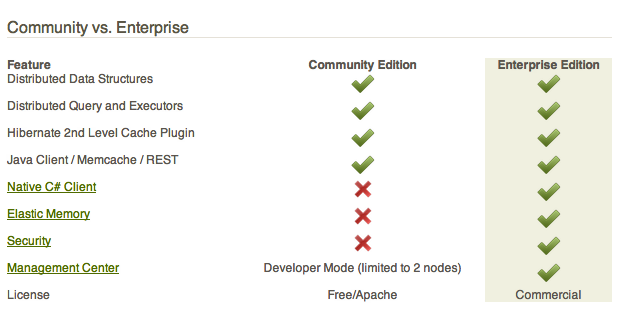
\includegraphics[scale=0.60]{hazelcast-editions.png}
For the purpose of this book we'll use the community edition. If your project relies on Maven, there is no need to install Hazelcast. Setting the dependencies is enough, see next chapter.

If your project is not relying on Maven, then make sure that the Hazelcast jar is added to the classpath, there is no need to install Hazelcast.

\section{Hazelcast and Maven}
Hazelcast is very easy to include in your Maven project without needing to install Hazelcast at all. Hazelcast can be found in the standard Maven repositories, so no need to added additional repositories to your Maven project. To include Hazelcast in your project, just add the following to your pom.xml:
\begin{lstlisting}[language=xml]
<dependencies>	
    <dependency>
      <groupId>com.hazelcast</groupId>
      <artifactId>hazelcast</artifactId>
      <version>2.5</version>
   </dependency>
</dependencies>
\end{lstlisting}
That is it. Make sure that you check the Hazelcast website to make use of the most recent version. After this dependency is added, Maven will automatically downloaded the dependencies needed. The lack of needing to install Hazelcast is something I really like because it saves up quite a lot of time, so we can spend that time doing more useful things.

\section{Configuring Hazelcast}
Hazelcast can be configured in different ways:
\begin{enumerate}
\item programmatic
\item XML-configuration file
\item Spring
\end{enumerate}
The programmatic configuration is the most rudimentary, the other mechanisms are build on top of it. In this book we'll use the xml configuration file. When you are running a Maven project; just add a resources directory under src/main/ and add a file 'hazelcast.xml'. The following shows an empty configuration:
\begin{lstlisting}[language=xml]
<hazelcast xsi:schemaLocation="http://www.hazelcast.com/schema/config
                               http://www.hazelcast.com/schema/config/hazelcast-config-2.5.xsd"
           xmlns="http://www.hazelcast.com/schema/config"
           xmlns:xsi="http://www.w3.org/2001/XMLSchema-instance">
</hazelcast>
\end{lstlisting}
This example also imports an XML schema (XSD) for validation and if you are using an IDE, you probably get code completion. To reduce the size of the examples in the book, the XSD import is left out.

In most of our examples we rely on multicast being enabled for member discovery. So if an XML configuration file is going to be used, it contains the following network configuration:
\begin{lstlisting}[language=xml]
<hazelcast>
    <network>
       <join><multicast enabled="true"/></join>
   </network>
</hazelcast>
\end{lstlisting}
See [chapter Cluster Configuration: Multicast] if multicast doesn't work or you want to know more about it. If you are using the programmatic configuration, then multicast is enabled by default.

In this book, the following approach is used to create a new Hazelcast instance:
\begin{lstlisting}[language=java]
public class Main {
    public static void main(String[] args){
        HazelcastInstance hzInstance = Hazelcast.newHazelcastInstance();
        ...
    }
}
\end{lstlisting}
The mechanism uses the following configuration file resolution chain:
\begin{enumerate}
\item first checks if the 'hazelcast.config' system property is set; if it is, then the value is used as path. This is useful if you want to choose on startup of the application which hazelcast configuration file should be used. The config option can be set by adding the following to the java command: '-Dhazelcast.config=<path to the hazelcast.xml>'. The value can be a normal file path, but can also be a classpath reference if it is prefixed with 'classpath:'. 
\item else it checks if there is a 'hazelcast.xml' in the working directory.
\item after that it check if there is a 'hazelcast.xml' on the classpath. 
\item and finally loads the default hazelcast configuration 'hazelcast-default.xml' that is part of the Hazelcast jar
\end{enumerate}

Another option to load a HazelcastInstance is to make use of programmatic configuration, e.g: 
\begin{lstlisting}[language=java]
public class Main {
    public static void main(String[] args){
        Config config = new Config();
        MapConfig mapConfig = new MapConfig();
        mapConfig.setName("testMap");
        config.addMapConfig(mapConfig);
        ...
        HazelcastInstance hzInstance = Hazelcast.newHazelcastInstance(config);
        ...
     }
}
\end{lstlisting}
The Hazelcast Config objects have fluent interfaces; meaning that the config object is returned when a config method is called, so that the next config method can be called. Programmatic configuration in my experience often is useful for testing purposes. 

\section{Wildcard configuration}
The Hazelcast xml configuration can contain configuration elements for all kinds of distributed data-structures: sets, executors, maps etc. For example:
\begin{lstlisting}[language=xml]
<hazelcast>
   <map name="testmap">
       <time-to-live-seconds>10</time-to-live-seconds>
   </map>
</hazelcast>
\end{lstlisting}
But what if we want to create multiple map instances using the same configuration? Do we need to define all these maps within the configuration file? This is impossible to do if you have a dynamic number of maps and you don't know up front how many need to be created. The solution to this problem is wildcard configuration. Hazelcast supports wildcard configuration for all data-structures. This makes it possible to use the single configuration for multiple instances. For example, we could configure the previous 'testmap' example with a time using a wildcard configuration like this:
\begin{lstlisting}[language=xml]
<hazelcast>
   <map name="testmap*">
       <time-to-live-seconds>10</time-to-live-seconds>
   </map>
</hazelcast>
\end{lstlisting}
Using a single asterisk (*) character any place in the name, different instances of Hazelcast data-structures can be configured by a single configuration. The wildcard configuration can be used like this:
\begin{lstlisting}[language=java]
     Map map1 = hzInstance.getMap("testmap1");
     Map map2 = hzInstance.getMap("testmap2");
\end{lstlisting}
The maps 'testmap1' and 'testmap2' both match 'testmap*' so they will use the same configuration.

One thing you need to watch out for are multiple configurations that match. Hazelcast will not thrown an error or log a warning. Also selecting the right configuration doesn't depend on the order of definition in the configuration file or based on the best fitting match. So really make sure that your wildcard configurations are very specific. One of the ways to do it is to include the package name:
\begin{lstlisting}[language=xml]
    <map name="com.foo.testmap*">
        <time-to-live-seconds>10</time-to-live-seconds>
    </map>
\end{lstlisting}
A map can be loaded calling 'Map map1 = hzInstance.getMap("com.foo.testmap1")'. 

\section{Multiple Hazelcast instances}
Normally you probably have a single Hazelcast Instance per JVM. But Multiple Hazelcast Instances can run in a single JVM. This is useful for testing.. [todo:Are there other usages?]
\begin{lstlisting}[language=java]
import com.hazelcast.config.Config;
import com.hazelcast.core.*;
public class MultipleMembers {
    public static void main(String[] args){
        HazelcastInstance hzInstance1 = Hazelcast.newHazelcastInstance();
        HazelcastInstance hzInstance2 = Hazelcast.newHazelcastInstance();
    }
}
\end{lstlisting}
When you start this multiple members, you see something like this in the output:
\begin{lstlisting}
Members [2] {
    Member [192.168.1.100]:5701 this
    Member [192.168.1.100]:5702
}
...
Members [2] {
    Member [192.168.1.100]:5701
    Member [192.168.1.100]:5702 this
}
\end{lstlisting}
As you can see there is a 2 member cluster created.

\section{Properties}
In the Hazelcast xml file properties can be included like this:
\begin{lstlisting}[language=xml]
<hazelcast>
    <properties>
        <property name="property-name">property-value</property>
    </properties>
</hazelcast>
\end{lstlisting}
For a full listing of available properties see the 'Advanced configuration' chapter in the Hazelcast documentation.

\section{Import}
[todo:hazelcast 3 is going to have imports]

\section{Variables}
[todo:hazelcast 3 is going to have variables] 

\section{Configure logging}
Hazelcast supports various logging mechanisms; 'jdk', 'log4', 'sl4j' or 'none' if you don't want to have any logging. The default is the logging is 'jdk': the logging that is part of the JRE. Logging can be set by using adding a property in the hazelcast xml configuration:
\begin{lstlisting}[language=xml]
<hazelcast>
    <properties>
        <property name="hazelcast.logging.type">log4j</property>
    </properties>
</hazelcast>
\end{lstlisting}
Or if you are using the programmatic configuration:
\begin{lstlisting}[language=java]
Config cfg = new Config() ;
cfg.setProperty("hazelcast.logging.type", "log4j");
\end{lstlisting}
But it can also be configured from the commandline 'java -Dhazelcast.logging.type=log4j'. If you are going to make use of 'log4j' or 'slf4j', make sure that the correct dependencies are included. One thing to watch out for; you can't override the logging configuration from the commandline if it already is specified in the Hazelcast configuration file.

If for whatever reason you are not satisfied with the provided mechanisms, you can always implement your own logging implementation by implementing the 'com.hazelcast.logging.LogListener'. See the Hazelcast reference manual for more information.
\section{Named Instances}

\section{Downloading example sources}
If you want to play around with the example sources of this book, check the following link:
TODO: Link to the source
